\documentclass[12pt, a4paper]{report}

% --- PREAMBLE: Packages and Settings ---
\usepackage[utf8]{inputenc} % Standard character encoding
\usepackage{geometry}       % Page margins
\geometry{a4paper, margin=1in}
\usepackage{graphicx}       % For including images
\usepackage{hyperref}       % For clickable links and TOC
\usepackage{setspace}       % For line spacing (e.g., \onehalfspacing)
\usepackage{caption}        % Better control over figure/table captions
\usepackage{enumitem}
\usepackage{subcaption}
\usepackage{booktabs}

\renewcommand{\bibname}{References}

% Link styling (removes ugly red boxes around links)
\hypersetup{
    colorlinks=true,
    linkcolor=blue,
    filecolor=magenta,      
    urlcolor=cyan,
    pdftitle={Report Title},
}

% --- TITLE PAGE INFO ---
\title{\textbf{Decidr}\\ \large An AI Tutor for Theory of Computation}
\author{Kien Nguyen \\ \textit{Library and Learning Services} \\ \textit{Sheridan College}}
\date{July, 2026}

% --- DOCUMENT BEGINS ---
\begin{document}

% Generates the title page
\maketitle

% Abstract (Optional)
\begin{abstract}
\noindent \textit{INFO 47546 - Theory of Computation} is considered one of the most challenging courses at Sheridan College due to the abstract nature of its concepts and the emphasis on rigourous mathematical proofs.~\\~\\
Despite efforts to promote existing tutoring services, student engagement remains limited, with only one student seeking tutoring support during the Spring 2026 academic term. We identify several potential barriers such as scheduling conflicts, uncertainty regarding available resources, and hesitation in seeking academic assistance.~\\~\\
To address these challenges, we developed \textbf{Decidr}, an AI tutor chatbot designed to provide accessible, on-demand academic support. By leveraging \textbf{Retrieval-Augmented Generation (RAG)} techniques with course-specific materials, Decidr provides students with contextualized explanations and guidance grounded in INFO 47546 course content. The system aims to complement existing tutoring resources by lowering barriers to academic support and enabling students to receive assistance at their own convenience.
\end{abstract}

% Generates the Table of Contents
\tableofcontents
\pagebreak

% --- MAIN CONTENT ---
\chapter{Introduction}
\textit{Theory of Computation} is a foundational subject in computer science that introduces students to abstract computational models, including finite automata, formal languages, and computability theory. Unlike many programming-oriented courses, students are required to reason about mathematical structures (sets, functions, finite automata, etc.) and construct formal proofs to demonstrate correctness. For many students, this course represents a significant transition from intuitive problem-solving approaches toward rigorous mathematical thinking.~\\~\\
At Sheridan College, tutoring services are available to students at no additional cost. Tutors with sufficient background were made available for students enrolled in the course. However, traditional tutoring models often require students and tutors to coordinate schedules, which may create barriers for students with competing academic or personal commitments. Additionally, some students may hesitate to seek help due to uncertainty about available resources, or concerns about asking questions they perceive as basic.~\\~\\
Recent advancements in large language models (LLMs) have created new opportunities for developing intelligent educational tools capable of providing immediate and personalized assistance. However, general-purpose AI systems such as ChatGPT, Gemini and Claude may provide inaccurate or inconsistent responses when answering course-specific questions. Further, due to the limitations in context window size, uploading all of the course notes to these systems proved to be inefficient and not helpful. Therefore, an effective educational assistant should be grounded in reliable course materials while maintaining the flexibility of conversational interaction.~\\~\\
In response to these challenges, we developed \textbf{Decidr}, an AI-powered tutor chatbot for \textit{INFO 47546 - Theory of Computation}. Decidr utilizes \textbf{Retrieval-Augmented Generation (RAG)} techniques to retrieve relevant information from course materials and incorporates this information into response generation, ensuring that explanations remain aligned with the curriculum.

\chapter{Background}
\section{Large Language Models}
\textit{Large Language Models (LLMs)} are a class of machine learning models designed to understand and generate human language \cite{ibm2026_1}. These models are usually based on the \textit{Transformer architecture} \cite{vaswani2017}, and are trained on large-scale text datasets (for example, the Internet) to learn patterns, relationships, and representations within the language.~\\~\\
Thanks to their ability to generate coherent and contextually relevant text, LLMs have shown strong performance across a wide range of \textit{Natural Language Processing (NLP)} tasks, including question answering, summarization, and conversational assistance.~\\~\\
The conversational capabilities of LLMs make them promising tools for educational applications. An LLM-based system can offer immediate responses, adapt explanations based on student questions, and support interactive learning experience. ~\\~\\
However, general-purpose LLMs have several limitations when applied to domain-specific context. Since the knowledge of an LLM is derived from its training data, general-purpose models may not contain the specialized information required for a particular course. Furthermore, updating an LLM's internal knowledge through additional training can be computationally expensive and impractical for frequently changing information. Additionally, LLMs can generate plausible but incorrect reponses when it doesn't have an answer (a phenomenon referred to as \textit{hallucination}). These limitations make it challenging to apply general-purpose LLMs directly to give course-specific information answers.
\section{Retrieval-Augmented Generation}
To address the limitations of LLMs outlined in the previous section, \textit{Retrieval-Augmented Generation (RAG)} approaches combine LLMs with external knowledge retrieval mechanisms, allowing models to access relevant information during response generation.~\\~\\
A typical RAG pipeline consists of two main stages: \textit{retrieval} and \textit{generation}. During the \textit{retrieval} stage, a user's query is used to identify relevant documents from an external knowledge base. These retrieved documents are then incorporated into the input prompt provided to the LLM. During the \textit{generation} stage, the LLM uses both the user's original query and the retrieved context to generate a response that is more accurate and grounded in the provided information.~\\~\\
By grounding responses in retrieved information, RAG reduces the likelihood of hallucination and allows LLM-based systems to incorporate domain-specific knowledge without requiring expensive model retraining. This makes RAG well-suited for applications such as educational assistants, where generated responses must remain consistent with specialized and potentially evolving course materials.
\begin{figure}[htbp]
    \begin{center}
        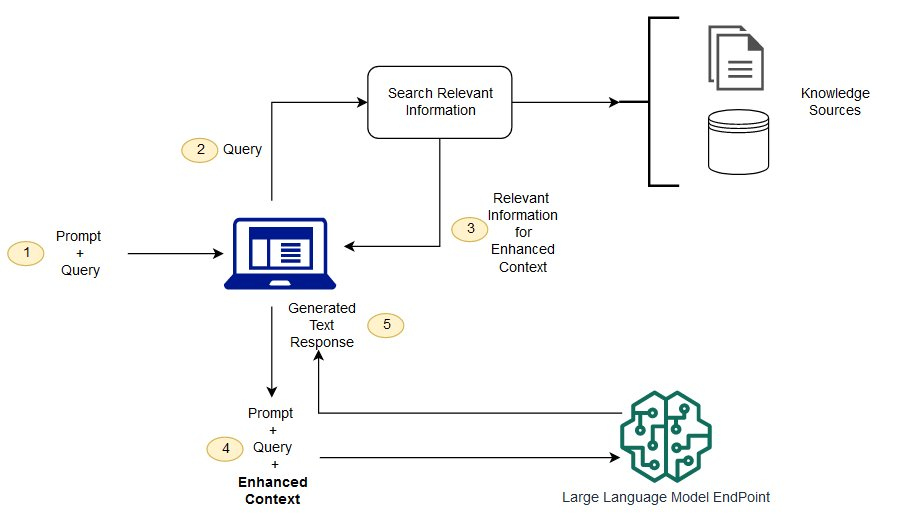
\includegraphics[width=0.8\linewidth]{photos/p1.png}
    \end{center}
    \caption{Architecture flow of Retrieval-Augmented Generation. Reprinted from \cite{aws_rag_image}.}
    \label{fig:rag_architecture}
\end{figure}
\section{Information Retrieval}
\textit{Information Retrieval (IR)} is a field in computer science concerned with finding documents or information that are relevant to a user's query. In RAG systems, the quality of retrieved documents directly influences the quality of the generated response. Modern retrieval systems generally employ either \textit{sparse} retrieval, \textit{dense} retrieval, or a combination of both (called \textit{hybrid} retrieval) \cite{ibm2026_2}.~\\~\\
In general, an information retrieval system works as follows:
\begin{itemize}
    \item \underline{Indexing:} Process and organize documents into a searchable index.
    \item \underline{Retrieval:} Given a user's query, rank indexed documents according to their estimated relevance and return the most relevant results.
\end{itemize}
The primary difference between \textit{sparse} and \textit{dense} retrieval lies in how documents and queries are represented during the indexing and retrieval stages.
\subsection{Sparse Retrieval}
Sparse retrieval methods represent documents as \textit{keyword-based representations}. Rather than capturing the semantic meaning of text, sparse retrieval algorithms rank documents based on the occurrence and importance of query terms. Consequently, these methods are particularly effective when a user's query closely matches the terminology contained within the indexed documents.~\\~\\
For example, if a user query contains the term ``deterministic finite automaton'', then sparse retrieval algorithms would strongly prioritize documents containing those exact words.
\subsection{Dense Retrieval}
Dense retrieval algorithms represent documents as \textit{vectors} (called \textit{embeddings}) that capture the documents' semantic meaning, rather than the exact words contained in them. This allows the retrieval system to identify relevant documents, even when different terminology is used.~\\~\\
For example, a query such as ``machines that accept strings'' may retrieve material discussing finite automata, even if those exact words do not appear.
\subsection{Hybrid Retrieval}
Sparse and dense retrieval exhibit complementary strengths. Sparse retrieval excels at exact terminology matching, while dense retrieval captures semantic similarity between related concepts. Consequently, many modern RAG systems employ hybrid retrieval strategies that combine both methods to improve retrieval accuracy.
\chapter{System Architecture}
\section{Overview}
% Explain how you conducted your research, gathered data, or approached the problem. 
The overall architecture of Decidr consists of \textit{two} primary pipelines: 
\begin{itemize}
    \item an offline \textit{indexing} pipeline, and 
    \item an online \textit{inference} pipeline
\end{itemize}
The offline \textit{indexing} pipeline processes course materials into a searchable knowledge base prior to deployment, while the online \textit{inference} pipeline retrieves relevant course content in repsonse to student queries and generates context-aware responses using an LLM.
\begin{figure}[htbp]
    \centering

    \begin{subfigure}[t]{0.48\linewidth}
        \centering
        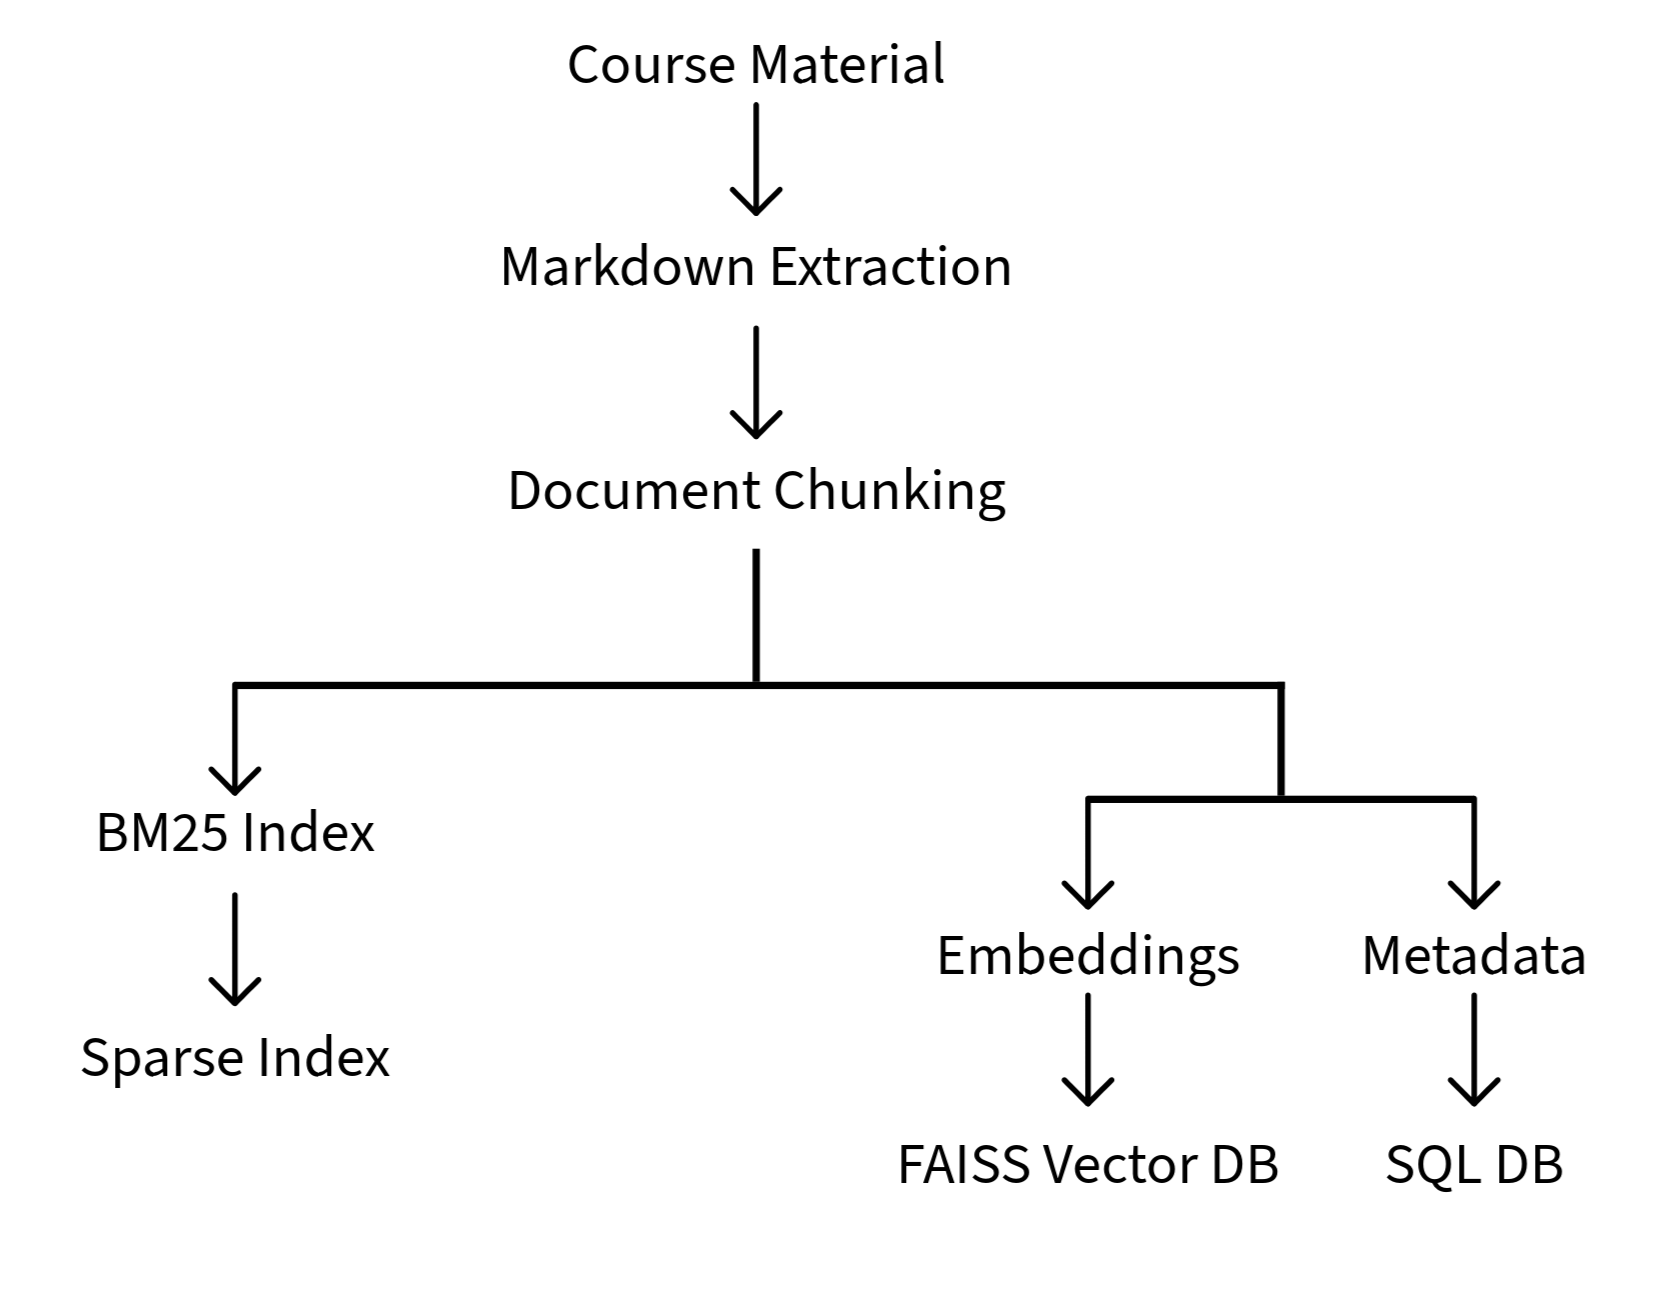
\includegraphics[width=\linewidth]{photos/p2.png}
        \caption{Offline indexing pipeline.}
        \label{fig:offline_pipeline}
    \end{subfigure}
    \hfill
    \begin{subfigure}[t]{0.48\linewidth}
        \centering
        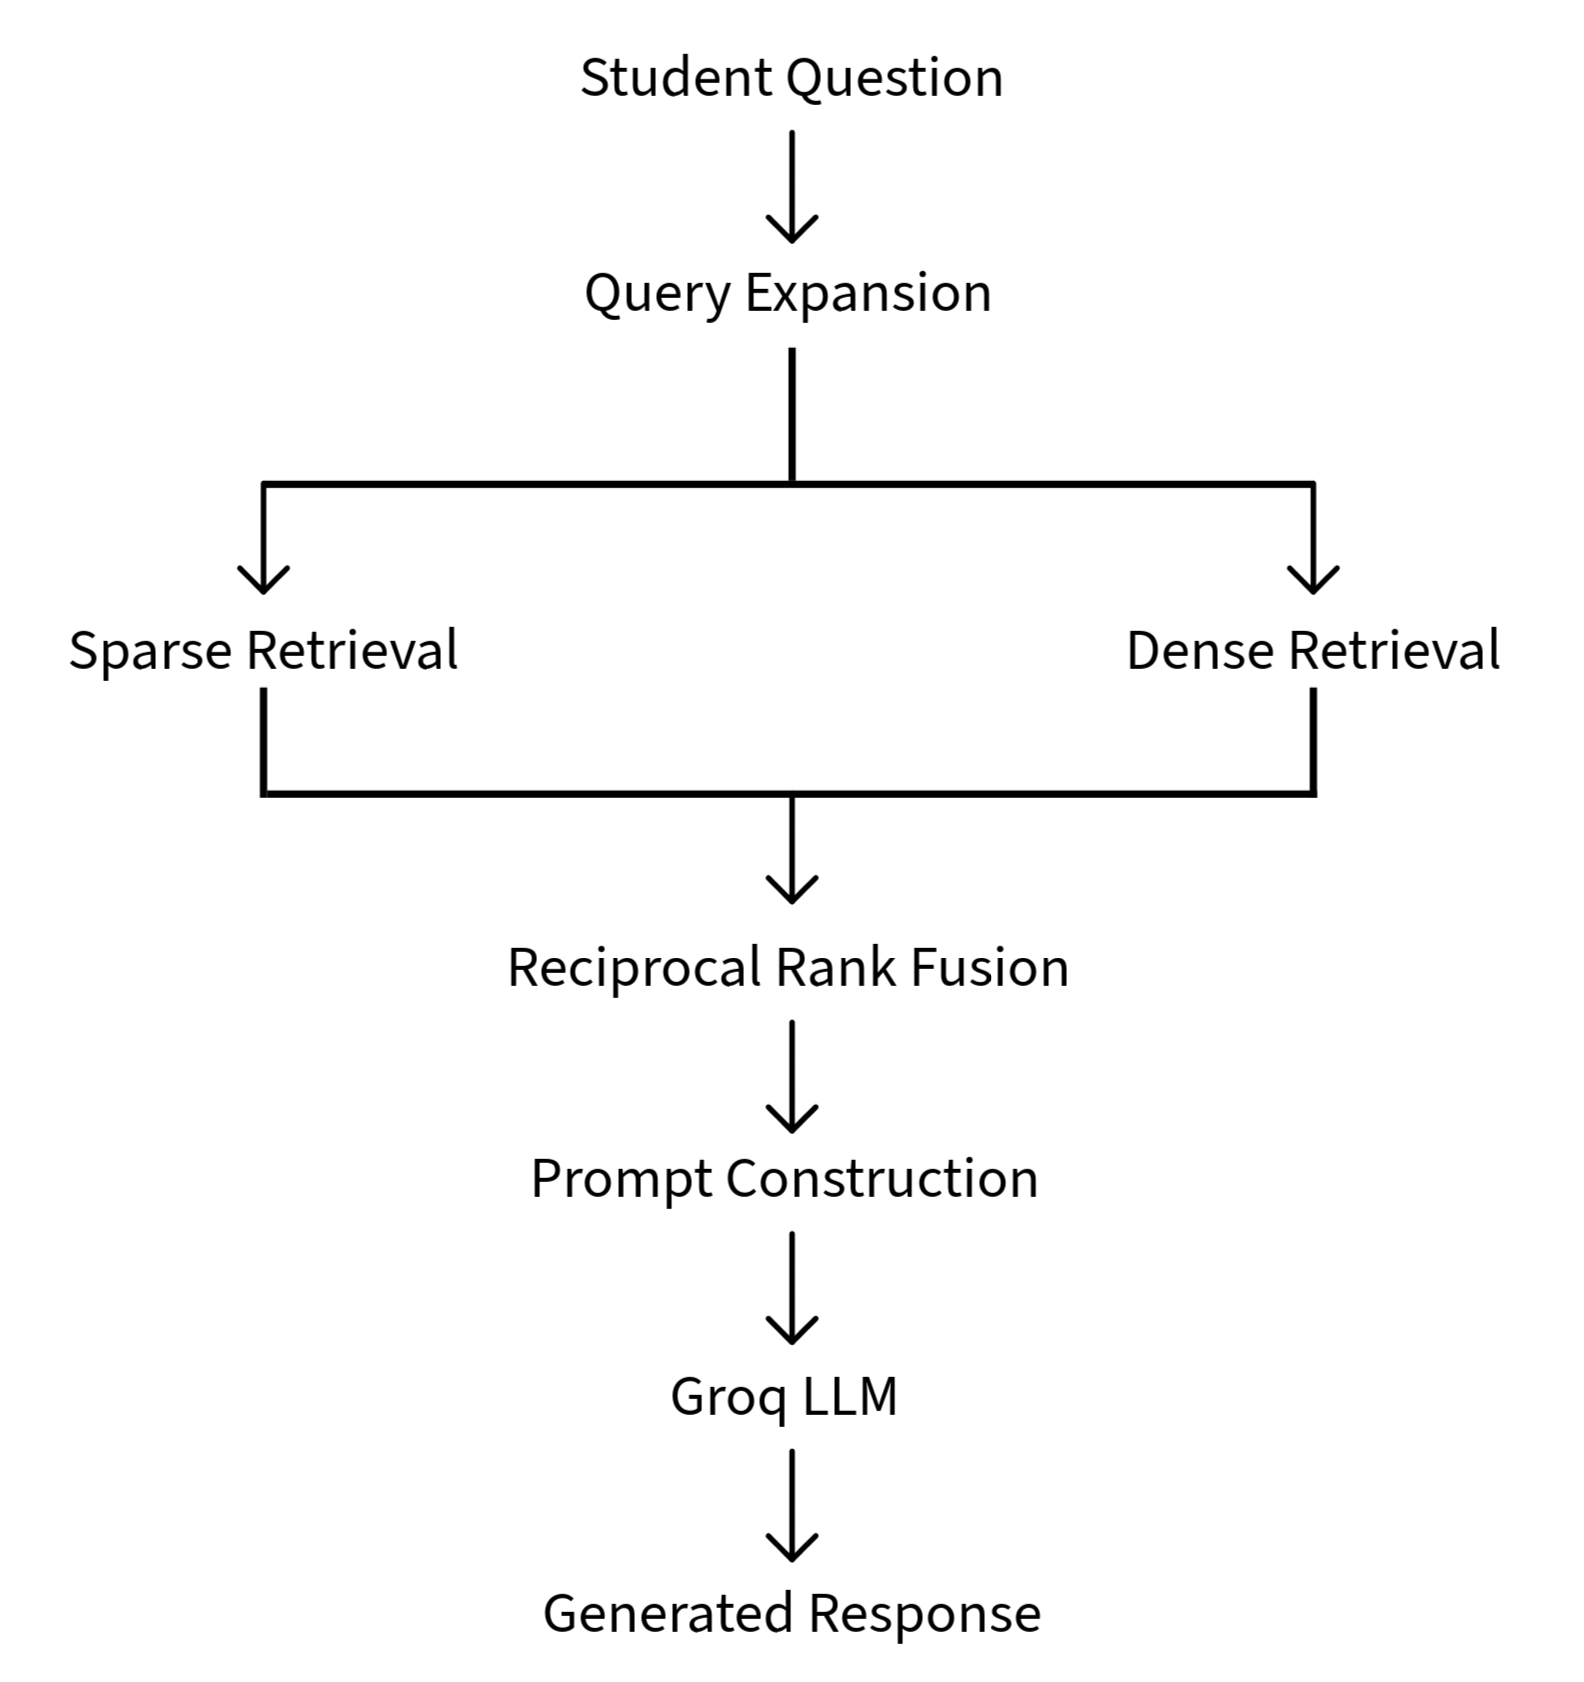
\includegraphics[width=\linewidth]{photos/p3.png}
        \caption{Online inference pipeline.}
        \label{fig:online_pipeline}
    \end{subfigure}

    \caption{Overview of Decidr's architecture. The offline pipeline constructs the searchable knowledge base, while the online pipeline retrieves relevant course materials and generates responses to student queries.}
    \label{fig:system_architecture}
\end{figure}

\section{Offline Indexing Pipeline}
Prior to deployment, these course materials are processed through an offline indexing pipeline to construct a searchable knowledge base. As illustrated in Figure~\ref{fig:offline_pipeline}, the pipeline consists of document extraction, document chunking, and the construction of both dense and sparse retrieval indices.
\subsection{Document Extraction}
Course materials for the course INFO 47546 consists of 12 PDF files, corresponding to the 12 weeks of content for the semester.~\\~\\
Although PDFs are well suited for document presentation, they do not explicitly encode the logical structure of the content, making reliable extraction of headings, paragraphs, mathematical expressions, and other elements challenging.~\\~\\
To facilitate downstream processing, the lecture notes were converted to Markdown format using \texttt{PyMuPDF4LLM}, an open-source Python library designed to extract text from PDF documents while preserving their logical structure for large language model (LLM) applications. This conversion preserves section headings and document hierarchy while producing a machine-readable format that simplifies subsequent chunking and indexing.
\subsection{Document Chunking}
After extraction, the Markdown documents are divided into smaller chunks before indexing. Splitting documents into smaller segments allows the retrieval system to return only the portions of the course notes that are most relevant to a student's question, rather than the entire lecture notes. This finer retrieval granularity reduces the amount of irrelevant context supplied to the language model, resulting in more focused and contextually relevant responses.~\\~\\
Decidr uses the \texttt{MarkdownHeaderTextSplitter} provided by LangChain, which preserves the document hierarchy by splitting content according to Markdown headings. As a result, each chunk remains associated with its corresponding lecture section and subsection, providing additional context during retrieval.
\subsection{Dense Index Construction}
Each document chunk is converted into a dense vector representation using the open-source \texttt{all-MiniLM-L6-v2} embedding model. These embeddings capture the semantic meaning of the text, allowing similar concepts to be retrieved even when different wording is used.~\\~\\
The resulting embedding is stored is stored in a FAISS vector index \cite{douze24} to support efficient similarity search. Alongside the vector index, a lightweight SQLite database stores the original document content and associated metadata (e.g., lecture week, section, and subsection). During retrieval, FAISS erturns the identifies of the most relevant vectors, while the SQLite database is used to recover the corresponding document chunks supplied to the language model.
\subsection{Sparse Index Construction}
In addition to dense retrieval, Decidr constructs a sparse retrieval index using the Okapi BM25 algorithm \cite{bm25okapi}. Each document chunk is tokenized and added to a BM25 corpus, enabling efficient keyword-based retrieval. Sparse retrieval complements dense retrieval by emphasizing exact terminology frequently used throughout Theory of Computation, such as deterministic finite automaton or Pumping Lemma.~\\~\\
The offline indexing pipeline is executed only when course materials are updated. Once the dense and sparse indices have been constructed, they are reused by the online inference pipeline to answer student queries in real time.
\section{Online Inference Pipeline}
Once the offline indexing pipeline has constructed the searchable knowledge base, Decidr is capable of answering student queries in real time. As illustrated in Figure~\ref{fig:online_pipeline}, the online inference pipeline consists of query preprocessing, hybrid retrieval, prompt construction, and response generation.
\subsection{Query Preprocessing}
When a student submits a question, the query first undergoes a preprocessing stage before retrieval. During this stage, common abbreviations and acronyms used throughout the Theory of Computation course are expanded using a predefined lookup table. For example, ``DFA'' is expanded to ``deterministic finite automaton'', while ``TM'' is expanded to ``Turing machine''.~\\~\\
This preprocessing step improves retrieval performance by ensuring that both dense and sparse retrieval algorithms operate on queries containing complete terminology, reducing ambiguity and improving the likelihood of retrieving relevant course materials.
\subsection{Hybrid Retrieval}
Following preprocessing, the expanded query is submitted to a hybrid retrieval pipeline consisting of both dense and sparse retrieval. These retrieval strategies operate independently before their results are combined.~\\~\\
For dense retrieval, the expanded query is converted into a dense vector representation using the \texttt{all-MiniLM-L6-v2} embedding model. The resulting embedding is compared against the FAISS vector index using inner-product similarity, returning the top-$k$ document chunks that are semantically similar to the student's query. By default, we set $k = 5$.~\\~\\
Simultaneously, the expanded query is tokenized and evaluated using the Okapi BM25 algorithm. Unlike dense retrieval, BM25 emphasizes exact keyword matching and is particularly effective when students use terminology that closely matches the course notes.~\\~\\
Finally, the ranked results produced by both retrieval methods are merged using \textit{Reciprocal Rank Fusion (RRF)} \cite{agarwal25}. Since dense and sparse retrieval produce scores on different scales, RRF combines the rankings rather than the raw similarity scores, producing a unified ranking that benefits from the complementary strengths of both retrieval strategies.
\subsection{Prompt Construction}
Following reciprocal rank fusion, the identifiers of the highest-ranked document chunks are used to retrieve the corresponding document content and metadata from the SQLite database. These reconstructed document chunks are then incorporated into the prompt provided to the language model.~\\~\\
The system prompt instructs the language model to answer questions using only the retrieved course materials whenever possible, maintain consistency with the terminology used throughout the course, and explicitly acknowledge when the retrieved context does not contain sufficient information to answer the question. By grounding the language model in retrieved course content, the system encourages responses that remain aligned with the curriculum while reducing unsupported or fabricated answers.
\subsection{Response Generation}
The completed prompt is submitted to a hosted large language model (\texttt{llama-3.3-70b-versatile}) through the Groq inference API. The language model synthesizes the retrieved course materials with the student's question to produce a coherent, contextually relevant response. The generated response is then returned through Decidr's conversational interface, allowing students to receive immediate, course-specific assistance.

\chapter{Iterative Development}
\section{Local LLM Inference}
During the initial stages of development, Decidr was designed to perform inference entirely on a local machine using a self-hosted large language model. Running the model locally eliminated dependency on external APIs, reduced operational costs, and provided complete control over the inference pipeline.~\\~\\
The initial prototype uses the \texttt{Llama3.1:8B} model by Meta, hosted through Ollama.~\\~\\
While the model was capable of producing coherent responses, inference latency proved to be a significant limitation. On a MacBook Pro equipped with Apple's M2 chip, generating a single response required approximately 15 seconds, resulting in an unsatisfactory user experience for an interactive tutoring application. Initially, we hypothesized that the limited memory available on the local machine was the primary performance bottleneck. To investigate this, the same model was deployed on a server equipped with substantially greater memory capacity. Surprisingly, inference time increased significantly, requiring approximately 30 seconds to generate a response. These experiments suggested that increasing available memory alone was insufficient to improve performance, and that inference throughput was instead constrained by computational resources available during model execution.~\\~\\
Since low response latency is critical for maintaining a conversational user experience, these observations motivated the exploration of alternative deployment strategies. In parallel, we also investigated whether the course-specific performance of the locally hosted language model could be improved through \textit{parameter-efficient fine-tuning (PEFT)}.
\section{Fine-tuned LLM}
In simple terms, \textit{parameter-efficient fine-tuning (PEFT)} is a family of techniques that adapt pre-trained language models to a specific task by updating only a small subset of the model's parameters while keeping the remaining parameters fixed. Compared with \textit{full fine-tuning} (where we update all of the model's weights), this approach substantially reduces the computational resources required for training \cite{ibmPEFT2026}. If successful, this approach could reduce the reliance on an external retrieval pipeline by incorporating course-specific knowledge directly into the language model. This would simplify deployment by requiring only the fine-tuned model to be hosted during inference.~\\~\\
We applied PEFT using the \textit{LoRA (Low-Rank Adaptation)} framework \cite{lora2021} to the \texttt{Llama3.1:8B} model in an effort to improve its performance on Theory of Computation questions while retaining the original model architecture. The model was fine-tuned on the \textit{TuringQ} dataset \cite{turingQ2024} using the Python library \texttt{Unsloth}.~\\~\\
The fine-tuned model demonstrated improved familiarity with Theory of Computation terminology and question formats present in the training dataset. However, its overall performance remained inadequate for a conversational tutoring system. In particular, the model frequently struggled to synthesize information distributed across multiple retrieved document chunks, occasionally producing responses that confused unrelated concepts or lacked logical coherence.~\\~\\
Furthermore, the \textit{TuringQ} dataset consists primarily of question-and-answer pairs collected from a variety of sources rather than Sheridan College's course materials. Consequently, although the model became more familiar with general Theory of Computation concepts, its responses often employed notation and terminology that differed from those used throughout the course. More importantly, the fine-tuned model continued to struggle with open-ended conceptual questions requiring multi-step reasoning, or the integration of information from multiple topics (e.g., ``What is the difference between a DFA and an NFA?''). These observations suggested that parameter-efficient fine-tuning alone was insufficient for producing reliable, course-specific tutoring responses.
\section{Adoption of RAG and Cloud Inference}
The experiments with local inference and parameter-efficient fine-tuning revealed two important limitations. First, adapting a language model through fine-tuning alone was insufficient to ensure that responses remained consistent with Sheridan College's course materials. Second, locally hosted models introduced significant latency, limiting their suitability for an interactive tutoring application.~\\~\\
Based on these observations, we shifted our focus from modifying the language model itself toward improving the information provided to the model during response generation. Rather than attempting to encode course-specific knowledge directly into model parameters, the final version of Decidr adopted a Retrieval-Augmented Generation (RAG) architecture, where relevant course materials are dynamically retrieved and provided as context to the language model.~\\~\\
Groq is a cloud inference provider specializing in high-performance execution of large language models through its custom \textit{Language Processing Unit (LPU)} architecture \cite{groq2024}. Unlike general-purpose GPUs, LPUs are designed specifically to accelerate the computational patterns involved in transformer inference, enabling high-throughput token generation and reduced response latency.~\\~\\
Since latency was identified as a major limitation of local deployment, Groq was selected as the inference provider for the final version of Decidr. By leveraging Groq's optimized inference infrastructure, Decidr was able to utilize a larger language model while maintaining the responsiveness required for an interactive tutoring application.
\section{Lessons Learned}
The iterative development process of Decidr highlighted several important considerations when developing LLM-based educational applications. Initially, we focused on improving the language model itself through local deployment and parameter-efficient fine-tuning. However, these experiments demonstrated that model adaptation alone was insufficient for producing reliable, course-specific responses.~\\~\\
One key observation was that retrieval quality plays a critical role in domain-specific applications. While fine-tuning improved the model's familiarity with certain concepts and terminology, it did not provide a reliable mechanism for incorporating updated or institution-specific course materials. In contrast, Retrieval-Augmented Generation allowed Decidr to ground responses in authoritative course content without requiring repeated model training whenever course materials changed.~\\~\\
Additionally, the experiments highlighted the importance of balancing model capability with deployment constraints. Larger language models generally provide stronger reasoning capabilities, but their computational requirements make local deployment challenging. By combining a capable hosted language model with an efficient retrieval pipeline, Decidr was able to achieve a balance between response quality, course alignment, and inference latency.~\\~\\
The following table summarizes the approaches evaluated during the development of this project:
\begin{table}[htbp]
\centering
\renewcommand{\arraystretch}{1.3}
\begin{tabular}{@{}llp{4.5cm}p{4.5cm}@{}}
\toprule
\textbf{Approach} & \textbf{Model} & \textbf{Strengths} & \textbf{Limitations} \\ 
\midrule
Local inference   & RAG + Llama 3.1 8B   & No API dependency, easy experimentation         & Slow inference, limited reasoning       \\ 
LoRA fine-tuning  & Llama 3.1 8B + LoRA & Better terminology familiarity               & Poor generalization, notation mismatch  \\ 
Final approach    & RAG + llama-3.3-70b & Course grounding, strong reasoning, low latency & Requires external inference API         \\ 
\bottomrule
\end{tabular}
\caption{Comparison of Modeling Approaches}
\label{tab:model-comparison}
\end{table}
% \chapter{Conclusion and Future Work}
% This project presented Decidr, an AI-powered tutoring chatbot designed to provide accessible academic support for \textit{INFO 47546 - Theory of Computation}. By combining Retrieval-Augmented Generation with hybrid information retrieval and a large language model, Decidr provides students with course-specific explanations grounded in official lecture materials.~\\~\\
% Although Decidr demonstrates the potential of RAG-based educational assistants, several improvements could further enhance its effectiveness, reliability, and maintainability. Currently, the retrieval corpus only contains lecture materials. Future work could expand the knowledge base to include additional course resources, such as exercises, assignments, and worked examples, allowing the system to provide more comprehensive support for students during problem-solving.~\\~\\
% The current query preprocessing stage relies on a manually constructed acronym lookup table to expand common Theory of Computation terminology. A potential improvement would be to replace this static approach with LLM-based query expansion, where the system generates multiple related search queries dynamically. This could improve retrieval performance for ambiguous or complex student questions.~\\~\\
% Additionally, the current retrieval pipeline could be enhanced through the integration of a re-ranking stage. While hybrid retrieval effectively combines semantic and keyword-based search, a learned re-ranking model, such as a cross-encoder, could further improve precision by evaluating the relevance of retrieved document chunks before they are provided to the language model.~\\~\\
% From a user experience perspective, future versions of Decidr could implement persistent conversation history using a database rather than relying on temporary session storage. This would allow students to resume previous tutoring sessions and enable more coherent multi-session interactions. Furthermore, evaluation tooling could be developed to monitor system performance over time, including retrieval metrics such as recall and generation metrics such as answer faithfulness, providing a more systematic approach for measuring improvements.~\\~\\
% Finally, the current prototype requires improvements in deployment security. Sensitive information, such as API keys, should be managed through environment variables or dedicated secrets management systems rather than being stored directly within the application code. This would make the system more suitable for production deployment.

\chapter{Conclusion and Future Work}

\section{Conclusion}

This project presented \textbf{Decidr}, an AI-powered tutoring chatbot designed to provide accessible academic support for \textit{INFO 47546 - Theory of Computation} at Sheridan College. The system addresses several challenges associated with traditional tutoring models, including scheduling constraints and uncertainty around seeking academic assistance.~\\~\\
Decidr combines Retrieval-Augmented Generation (RAG), hybrid information retrieval, and a large language model to provide students with course-specific explanations grounded in official lecture materials. Through the use of dense and sparse retrieval techniques, relevant course content can be identified and incorporated into the language model's context, improving the reliability and consistency of generated responses.
% The iterative development process demonstrated that building an effective educational LLM system requires careful consideration of multiple factors, including retrieval quality, model capability, and inference efficiency. Initial experiments with local inference and parameter-efficient fine-tuning revealed the limitations of relying solely on model adaptation for domain-specific applications. The final architecture, which combines RAG with a capable hosted language model, provided a more effective balance between response quality, course alignment, and latency.~\\~\\

\section{Future Work}
Although Decidr demonstrates the potential of RAG-based educational assistants, several improvements could further enhance its effectiveness, reliability, and maintainability.~\\~\\
Currently, the retrieval corpus contains only lecture materials. Future work could expand the knowledge base to include additional course resources, such as exercises, assignments, and worked examples. Incorporating these materials would allow Decidr to provide more comprehensive assistance, particularly for students seeking help with problem-solving and practice questions.~\\~\\
The current query preprocessing stage relies on a manually constructed acronym lookup table for expanding common Theory of Computation terminology. A potential improvement would be to replace this static approach with LLM-based query expansion, where multiple related queries are generated dynamically. This could improve retrieval performance for ambiguous or complex student questions.~\\~\\
Furthermore, the retrieval pipeline could be enhanced through the addition of a re-ranking stage. While hybrid retrieval combines the complementary strengths of dense and sparse retrieval, a learned re-ranking model, such as a \textit{cross-encode}r, could improve precision by evaluating the relevance of retrieved document chunks before they are provided to the language model.~\\~\\
From a user experience perspective, future versions of Decidr could implement persistent conversation history using a database rather than temporary session storage. This would allow students to resume previous tutoring sessions and enable more coherent multi-session interactions. Finally, evaluation tooling could be developed to monitor system performance over time, including retrieval metrics such as recall and generation metrics such as answer faithfulness.
\begin{thebibliography}{9}

\bibitem{ibm2026_1}
Struker, C. ``What are large language models (LLMs)?''. \textit{IBM}, \url{https://www.ibm.com/think/topics/large-language-models}

\bibitem{vaswani2017} 
Vaswani, A., Shazeer, N., Parmar, N., Uszkoreit, J., Jones, L., Gomez, A. N., Kaiser, L., Polosukhin, I. ``Attention Is All You Need''. \textit{arXiv preprint}, 2017, arXiv:1706.03762.

\bibitem{aws2026}
Amazon Web Services (AWS). ``What is RAG (Retrieval-Augmented Generation)?''. \textit{Amazon Web Services} \url{https://aws.amazon.com/what-is/retrieval-augmented-generation/#how-does-retrieval-augmented-generation-work--1xobboj}

\bibitem{aws_rag_image}
Amazon Web Services (AWS). ``Visualization of a RAG system''. [Online Image]. \textit{Amazon Web Services}, 2026. \url{https://aws.amazon.com/what-is/retrieval-augmented-generation/#how-does-retrieval-augmented-generation-work--1xobboj}

\bibitem{ibm2026_2}
Murel, J., Syed, M. ``What is information retrieval?''. \textit{IBM}, \url{https://www.ibm.com/think/topics/information-retrieval}

\bibitem{bm25okapi}
Park, E. ``Understanding Okapi BM25 - Document Ranking algorithm''. \textit{Medium}, 2025. \url{https://medium.com/@readwith_emma/
understanding-okapi-bm25-document-ranking-algorithm-70d81adab001}

\bibitem{douze24}
Douze, M., Guzhva, A., Deng, C., Johnson, J., Szilvasy, G., Mazaré P-E., Lomeli, M., Hosseini, L., Jégou, H. ``The Faiss library''. \textit{arXiv preprint}, 2024, 	arXiv:2401.08281.

\bibitem{agarwal25}
Agarwal, S. ``Search: Reciprocal Rank Fusion - Your Search Engine's Secret Weapon''. \textit{Medium}, 2025. \url{https://shivamagarwal7.medium.com/search-reciprocal-rank-fusion-9735dcd1906d}

\bibitem{ibmPEFT2026}
Belcic, I., Stryker, C. ``What is parameter-efficient fine-tuning (PEFT)?''. \textit{IBM}, 2025. \url{https://www.ibm.com/think/topics/parameter-efficient-fine-tuning}

\bibitem{lora2021}
Hu, E. J., Shen, Y., Wallis, P., Allen-Zhu, Z. Li, Y., Wang, S., Wang, L., Chen, W. ``LoRA: Low-Rank Adaptation of Large Language Models''. \textit{arXiv preprint}, 2021, arXiv:2106.09685.

\bibitem{turingQ2024}
Zahraei, P., Asgari, E. ``TuringQ: Benchmarking AI Comprehension in Theory of Computation''. \textit{arXiv prepreint}, 2024, arXiv:2410.06547

\bibitem{groq2024}
Groq. ``What is a Language Processing Unit?''. \textit{Groq}, 2024, \url{https://cdn.sanity.io/files/chol0sk5/production/4e3e6966d98da9ef4bfd9834dbfc00921da58252.pdf}

\end{thebibliography}


% --- APPENDIX ---
% \appendix
% \chapter{Supplementary Data}
% Include raw data, extra charts, lengthy code blocks, or survey questionnaires here so they don't clutter the main body of the report.


\end{document}